\onehalfspacing 
\label{chapter2}
\section{Variety and Repetition}
In response to Kyle Adams' \textit{Music Theory Online} article ``Aspects of the Music/Text
Relationship in Rap,'' Justin Williams remarks on a significant phenomenological development
in rap music production, following the genre's move from the turntable, to the studio, and 
even more recently to the Digital Audio Workstation (DAW). He writes:
    \begin{quote}
        \small ``In terms of rap music recordings, the idea of a completely fixed loop is 
        largely fictitious. There may be a set of layers which we could term the `basic beat'
        which repeats intact for certain durations of time, but one would be hard-pressed to
        find an entire musical complement that stays the same throughout. Rap music’s layers
        will more often than not fluctuate throughout a given song, with sonic additions and
        subtractions, manipulations of digital samples, and even sharp changes in aspects of
        the basic beat.''\footnote{
            \cite{justinawilliamsBeatsFlowsResponse2009}. It is worth noting that Adams does 
            not dispute the occurrence of development within an accompaniment as a phenomenon,
            but he does maintain that the unchanging elements of the beat function as ``primary
            accompanimental layers'' (See \cite{kyleadamsPeopleInstinctiveAssumptions2009}.)}
    \end{quote}
Repetition and variation are equally essential within the musical lexicon of rap instrumentals.
Adams notes that even as the locus of rap music-making moved into the studio, producers remained
adherent to the break-beat based origins of the genre, and so structural elements of the hip-hop
beat tend to repeat within a four to eight bar, often simple quadruple metrical space. At the same
time, Williams' observations point towards a preference for variation within repetition, made 
feasible by newer technologies for sampling, manipulating, and composing with pre-recorded digital
materials.

Whether the hip-hop beat is primarily repetitive or primarily developmental is indeterminate
because both variables exert influence over the creative process; a question of more value is
how different producers use these phenomena to aesthetic or rhetorical ends. To invoke Loren
Kajikawa's notion of sounding, variety and repetition factor into how ``rap artists produce 
(and listeners interpret) musical meanings at the level of the song.''\footnote{
    \autocite[2]{lorenkajikawaSoundingRaceRap2015}.} 
Although Kajikawa focuses on the sounding of racial and gender identities, his critical apparatus
may also extend to producers' use of music to identify with or against their perception of a 
hip-hop mainstream. I therefore argue that underground producers make beats that code themes and
identities in conversation with the hip-hop mainstream while rappers simultaneously declare allegiance
to the underground within their flow. Because, as Kajikawa notes,``rap has cultivated a mainstream
audience\textellipsis by promoting highly visible (and often controversial) representations of 
black masculine identity,''\footnote{
    \autocite[5]{lorenkajikawaSoundingRaceRap2015}.} 
the hip-hop underground operates as a  space to subversively play with these representations.

What I call the \emph{underground} signifies a space where multiple approaches to the sonic
construction of identity exist.\footnote{
    A more in-depth discussion of my definition and limitations of the term can be found in 
    Section~\ref{undergrounddeflims}.} 
Rather than being unified by a musical style, underground hip-hop is unified by a culture 
of listening. This definition is vague because underground is an elusive term, yet it holds
importance because it represents an imagined community with which rappers, producers, and
listeners identify.\footnote{
    Scholars including Williams and Joseph G. Schloss, have theorized hip-hop culture as 
    an imagined community, a from Benedict Anderson's writings on national identities. 
    Such communities have inhabitants who ``will never  know most of their fellow
    members, meet them, or even hear of them, yet in the minds of each lives the image of
    their  communion'' (see \autocite[6]{benedictandersonImaginedCommunitiesReflections2006}.).

    Hip-hop studies scholars use the term to create cohesion to discourse within hip-hop. 
    Both Schloss and Williams describe overlapping spheres of association, influence, and
    reference communicated through songs, beats, and albums. They argue hip-hop's imagined
    community therefore communicates and understands structures of tradition, history, and
    identity through these works. (see \autocite[4]{josephgschlossMakingBeatsArt2004}, and
    \autocite[12--13]{justinawilliamsRhyminStealinMusical2013}.)}

In this chapter, I argue that underground hip-hop producers sound undergroundness in beats
as a way to communicate the emcee's alternative identity to listeners. I base this argument
in transcriptions that illustrate developmental and repeating elements within the musical 
texture. My four case studies demonstrate two ways in which this occurs: first, underground
producers often deviate from mainstream formal models for rap music, and second, they rely
on methods of sample and loop manipulation such as \emph{resampling (or recomposing)}, 
\emph{choking}, \emph{glitching} and \emph{slipping} to create variety. These methods
prioritize an overarching aesthetic of diversity within the musical texture, linking
underground production to Olly Willson's heterogeneous sound ideal of African American 
music.\footnote{
    \cite{ollywilsonHeterogeneousSoundIdeal1992}.}

%\clearpage
\section{Methods of Transcription and Analysis} \label{methodsoftranscription}
I use transcription in this chapter\textemdash indeed, overall in this project\textemdash
despite  knowing that it introduces a level of abstraction from both the musical practice
and perceptual experience of my hip-hop repertory. Scholars such as Joseph G. Schloss 
have meaningfully analyzed hip-hop production while eschewing transcription altogether
on ethical and aesthetic grounds.\footnote{
    \autocite[13--15]{josephgschlossMakingBeatsArt2004}.} 
Others, like Kajikawa and Adam Krims, have employed methods of transcription that move
away from standard notation in the Western Classical tradition.\footnote{
    \autocite[29--30 and 36--37]{lorenkajikawaSoundingRaceRap2015};
    \autocite[105--110]{adamkrimsRapMusicPoetics2000}.} 
Still others, including Adams and Robert Komaniecki, rely primarily on standard notation
in order to present their arguments within traditional spheres of music-theoretical
discourse.\footnote{
    \cite{kyleadamsMetricalTechniquesFlow2009}; 
    \cite{robertkomanieckiAnalyzingCollaborativeFlow2017}.} 
Each approach holds its own merit, and each privileges a different audience: the creator,
the listener, and the academic.

Although I understand Schloss and others' reticence to transcribe rap music, my choice
to do so grows out of the mode of deep listening requisite to creating a transcription.
By using transcription, I do not aim to apply ``the tools of notation and analysis 
developed for the study of Western Classical music\textellipsis uncritically to rap
music.''\footnote{
    \autocite[12]{lorenkajikawaSoundingRaceRap2015}.}
Instead, I offer them as a subjective realization of my ``living inside'' the musical
object for a time.\footnote{
    \autocite[200]{peterwinklerWritingGhostNotes1997}.} 
Transcription therefore offers the best method of communicating my experience within
a written medium.

I use both standard and non-standard styles of transcription in this chapter to distinct
ends. First, I use tables that I call ``roadmaps'' to provide an overview of musical form,
noting the  relationship between sections, samples, and durations.\footnote{
    Each roadmap in the chapter has a corresponding expanded version that details the 
    function and relationship of each instrumental layer and counting durations by 
    samples. These expanded versions can be found in the appendix beginning on
    p.~\pageref{appendix:fullroadmaps}.} 
I also pay special attention to when producers create variety within the musical texture
using one of the four methods listed above and defined below. Second, I use standard
notation to create a musical ``snapshot'' of the beat at distinct points in the texture.
These snapshots allow me to discuss the function of particular musical layers and also to
more closely analyze the methods of creating variety outlined in the roadmaps. Using staff
notation requires a certain reduction of the rhythmic and textural complexity of my pieces,
but I use these snapshots in an effort to draw out the moments that cannot be easily notated
within them.

As my roadmaps show, underground producers play with expectations for form in mainstream
hip-hop, typically avoiding the \emph{verse-hook} formal model. Ben Duinker defines 
verse-hook form in hip-hop as an analog to \emph{verse-chorus} form in popular music, and
he shows that hip-hop's assimilation to mainstream popular culture has correlated with
increased use of this model.\footnote{
    \autocite[105]{benduinkerSongFormMainstreaming2020}.}\label{duinkerhookdef}
At the same time, he differentiates verse-hook from verse-chorus on account of the means
by which hooks fulfill the role of refrains.\footnote{
    Duinker states that hooks, unlike choruses, are not paired into units David Temperley
    labels ``verse-chorus units'' or VCUs, nor do they exhibit the same differentiating
    features that Temperley suggests choruses in rock songs do
    (see \autocite[159\textit{ff}]{davidtemperleyMusicalLanguageRock2018}.)}
Nevertheless, the correlation between verse-hook form and the mainstreaming of rap music
in popular culture offers underground producers a model of song form with which to converse
in their  effort to create hip-hop in dialogue with expectations.

Underground producers tend to make beats that articulate the section types Duinker identifies:
hooks, instrumentals, and ``looser-organized'' sections.\footnote{
    \autocite[95--101]{benduinkerSongFormMainstreaming2020}.} 
Though admitting some ambiguity, I define formal sections in this chapter based on production
rather than just text because many of the case studies are through-composed. How a producer 
chooses to order musical material can either clarify or contrast the form projected by the
vocal performance. Defining formal sections using production, then, becomes helpful for
showing when heterogeneity manifests through formal contrast, and when producers use samples
and loops to divide an emcee's through-composed text.

My snapshots show how underground producers prefer variety within formal sections to unaltered
loops and samples. Duinker notes that within verses particularly, the looped sequence of the beat
can change gradually through the introduction or subtraction of loops that are generally one, two,
or four measures in length through \emph{layering}. \footnote{
    \cite[96]{benduinkerSongFormMainstreaming2020}.} 
While underground producers also use layering, the techniques I define in the following
paragraphs create changes to the texture that are sharper and more drastic than layering.

Underground producers introduce changes within the beat using techniques that mimic the 
live, improvisatory roots of hip-hop; these are the methods of alteration I introduced 
above.  In order to present my close readings of each case study below, I will define 
\emph{resampling (or recomposing)}, \emph{choking}, \emph{glitching}, and \emph{slipping}, 
in the paragraphs that follow.

I use \emph{resampling} to refer to the changes producers make to a sample that still presents it 
as an intact whole. The term comes from a function several samplers and DAWs share, where a producer
can trigger audio on a track or pad, then engage processing effects that allow them to manipulate 
pitch, timbre, or dynamics in real time while the result of their manipulations is captured on a
second track or pad. \textit{Recomposing} is the term's corollary to describe changes made by
producers who use live-tracked elements in their mix; producers recompose a loop by adding new
pitch and rhythmic material, or by altering the loop's timbre in some conspicuous way.

I define \emph{choking} as instances where producers mute a portion of the loop or sample
completely, cutting it off as a sound source. While layering deals with gradual substraction
of sounds, a choke happens within the length of a sample or loop. Chokes can occur at lengths
perceptually experienced as a beat, as well as rhythmic durations below the level of meaningful
notation. Both resampling and choking challenge the perception that a loop has repeated without
completely disrupting its function as a loop.

\label{glitch}
By contrast, \emph{glitching} and \emph{slipping} each challenge repetition due to their marked 
change to the samples and loops. Producers \emph{glitch} a sample or loop by ``chopping'' out
a portion of audio within the time-span of one beat and repeating it to extend beyond one beat; 
this interrupts the texture in a way comparable to scratching a vinyl record would in turntabling. 
By contrast, producers \emph{slip} a sample in two more subtle ways: they either use samples with
slightly varied loop lengths, which, over long periods of time, slip apart, widening the gaps
between them; or, alternatively, they slip samples through re-triggering onsets rather than
looping them, adding micro-rhythmic delay as an expressive technique.ng them, adding micro-rhythmic 
delay. Both methods create a disalignment of sample and loop onsets.

As my analyses below demonstrate, underground producers use these compositional techniques to
create  variety within the sonic profile of their beats. In both sample-based and live-tracked
approaches to beatmaking, I examine case studies that illustrate the internal and formal variety
producers construct in dialogue with the emcee's vocal delivery. I aim to show that producers 
use these techniques to create variety within the sonic profile of their beats, and that their
alterations to samples, loops, and form introduce heterogeneity to the work, articulating an 
underground aesthetic in comparison to mainstream approaches.

%\clearpage
\section{Sample-Based Case Studies} \label{samplebased}
The contemporary practice of sample-based beatmaking links back to hip-hop's origins, echoing
the practice of looping breakbeats on the instrumental b-sides of vinyl records pioneered by
DJs like Kool Herc and Grandmaster Flash.\footnote{
    \autocite[51]{triciaroseBlackNoiseRap1994}.} 
Because producers who sample do not need to be multi-instrumentalists to create a full musical
texture, sample-based  beatmaking democratizes music production; but, furthermore, it situates
hip-hop within lineages of sound. Tricia Rose likens the ingenuity of hip-hop production to other
forms of black creativity, where making something good often involves ``making\textellipsis out
of the scraps\textemdash creating a delicacy of the undesirable, discarded parts.''
    \footnote{\autocite[264]{triciaroseHipHopWarsWhat2008}.} 
In the underground, the process of selecting a sample, re-contextualizing it in a new space, and
exploring the full extent of variety it may hold seems to be a look backwards to this tradition 
and, thus, a way of honoring a broader history of the ingenuity of black Americans.

\phantomsection
\subsection*{\centering MF DOOM's ``One Beer''}  
\addcontentsline{toc}{subsection}{MF DOOM's ``One Beer''}

    \begin{table}[ht]
        \centering
            \begin{tabular}{|c|c|c|c|l|}
                 \hline
                  Section         & Timecode & Duration & Sample              & Note                    \\ \hline
                  Intro           & 0:00     & 8 Bars   & ``Huit Octobre'' I  & Choked in Bar 8         \\ \hline
                  Verse 1A        & 0:20     & 16 Bars  & ``Huit Octobre'' II &                         \\ \hline
                  Verse 1B        & 1:02     & 16 Bars  & ``Huit Octobre'' II & Choked in Bar 0.4       \\ \hline
                  \sout{Hook}     & 1:43     & 8 Bars   & ``Huit Octobre'' I  & Choked in Bar 8.3-4     \\ \hline
                  Verse 2B        & 2:03     & 8 Bars   & ``Huit Octobre'' II & Choked in Bar 0.4, 8.4  \\ \hline
                  \sout{Verse 2C} & 2:24     & 16 Bars  & ``Huit Octobre'' II & Choked in Bar 0.4       \\ \hline
                  Skit            & 3:06     & 26 Bars  & \textit{Spider-Man} & Resampling, drum improv \\ \hline
             \end{tabular}
        \caption{Condensed roadmap to MF DOOM and Madlib's ``One Beer.''}
        \label{tab:onebeer}
    \end{table}

Madlib produces ``One Beer'' using two samples from the French funk band Cortex's ``Huit Octobre
1971.'' Outlined in Table~\ref{tab:onebeer}, he sequences these two samples with a normative 
approach to form, in contrast to DOOM's through-composed verse. Madlib starts ``One Beer'' with
an eight-bar introduction built from the first sample, followed by two sixteen-bar verse-parts
built from the second. He then switches back to the first sample, making space for a hook, 
but DOOM's verse continues over this projected boundary. After eight bars, the second sample
re-enters for another twenty-four, creating a nearly parallel second verse area for DOOM. The
two project contrasting forms in their respective roles as producer and rapper, and the dissonance
between the two creates heterogeneity between the text and the instrumental.

Madlib also introduces heterogeneity within the beat itself, primarily through disparities
in the selection of sampled portions from ``Huit Octobre.'' His first selection, 1:58-2:09
of  Cortex's recording, is pitched up slightly sharper than a whole step, tonicizing F-sharp.
Shown in Figure~\ref{fig:onebeerintro}, the sample grooves in a triplet eighth swing, featuring
synth and bass  in octaves arpeggiating I$^{b7}$ and a skeletal drum part emphasizing backbeats.
When the track returns to the first sample, the musical elements grant the sample a 
hook-like function.

    \begin{figure}[ht]
        \centering
        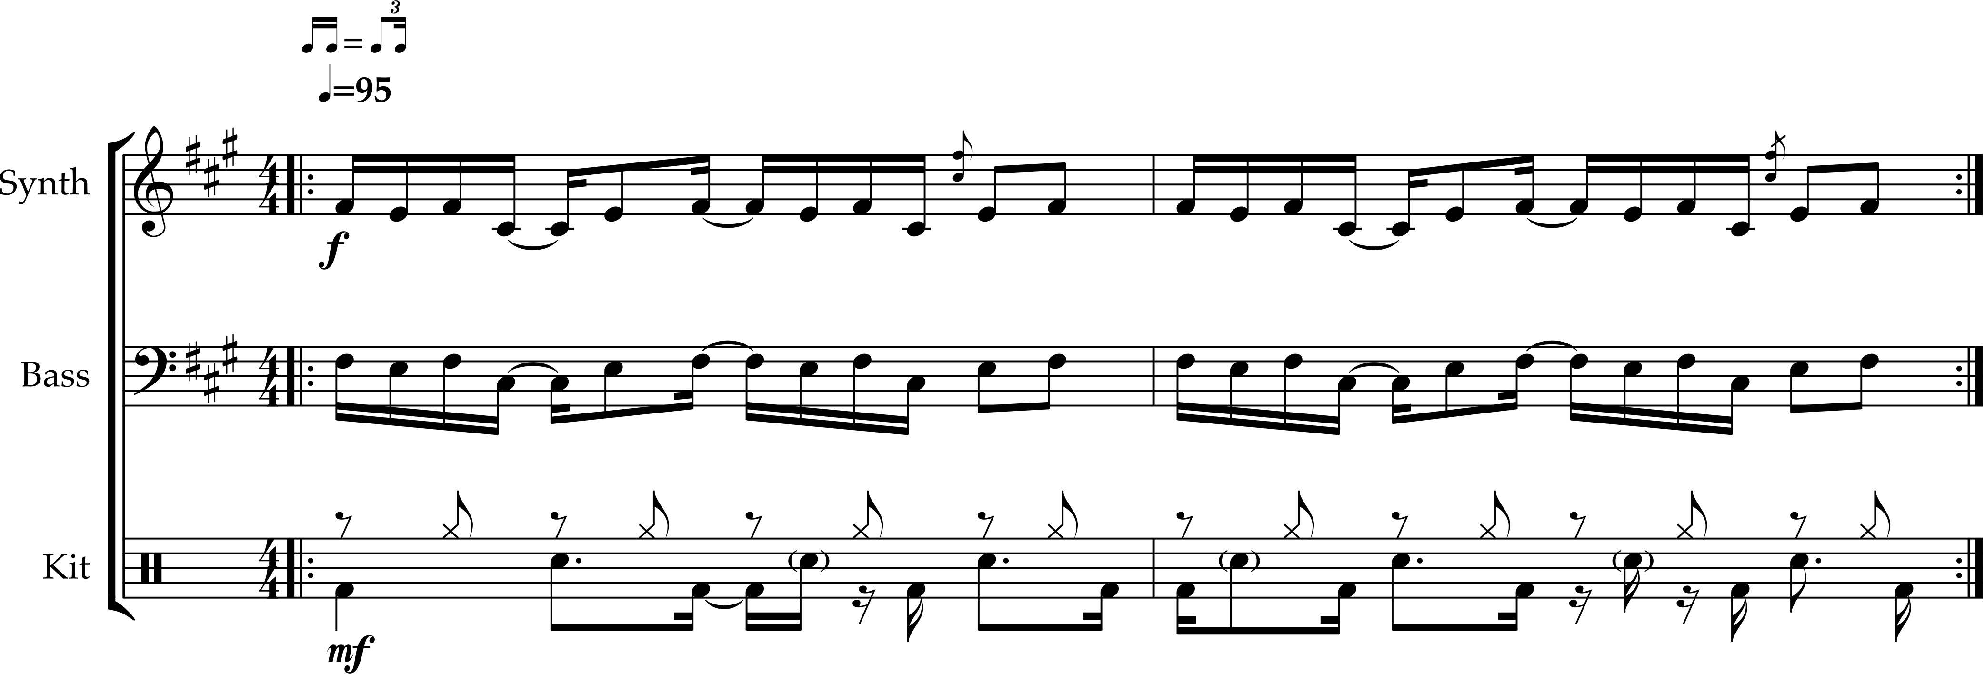
\includegraphics[width=\textwidth]{images/figures/chp 02/000019onebeerintro.pdf}
        \caption{Snapshot of Madlib's first sample in ``One Beer,'' 0:00--0:19.}
        \label{fig:onebeerintro}
    \end{figure}

The first sample sounds like a hook for two reasons. First, it is texturally distinct from
the sample  which underscores the verse portion of ``Huit Octobre,'' the primary instrumental
criterion Duinker identifies for distinguishing hooks from verses.\footnote{
    \autocite[99]{benduinkerSongFormMainstreaming2020}.}
Second, it is created from a shorter, more singularly-focused musical idea. Its harmony, which
Adams  typifies as \emph{repetitive}, is created from two arpeggiations of a one-measure idea
in rhythmic unison, only with slightly varied articulations in each statement.\footnote{
    \cite{kyleadamsHarmonicSyntacticMotivic2020}. The three categories Adams provides for 
    harmony in hip-hop are repetitive, oscillating, and expansional, all of which I touch on
    throughout the course of this chapter.} 
Overall, this section is sparser in texture and musical material and sounds like a point of
arrival.

Madlib contrasts the first sample with his selection of the second, 0:23-0:25 of the Cortex
recording. Although also pitched up slightly sharper than a whole step, this portion slows 
to 92 bpm from 95 bpm  and has a straight rhythmic feel. As Figure~\ref{fig:onebeermain} 
shows, both the overall musical texture and harmonic content of this sampled section have 
thickened in comparison to the first. Playing distinct and more typical instrumental roles,
the bass and synth underscore a vocal part, and the three create new oscillating harmonies.

    \begin{figure}[ht]
        \centering
        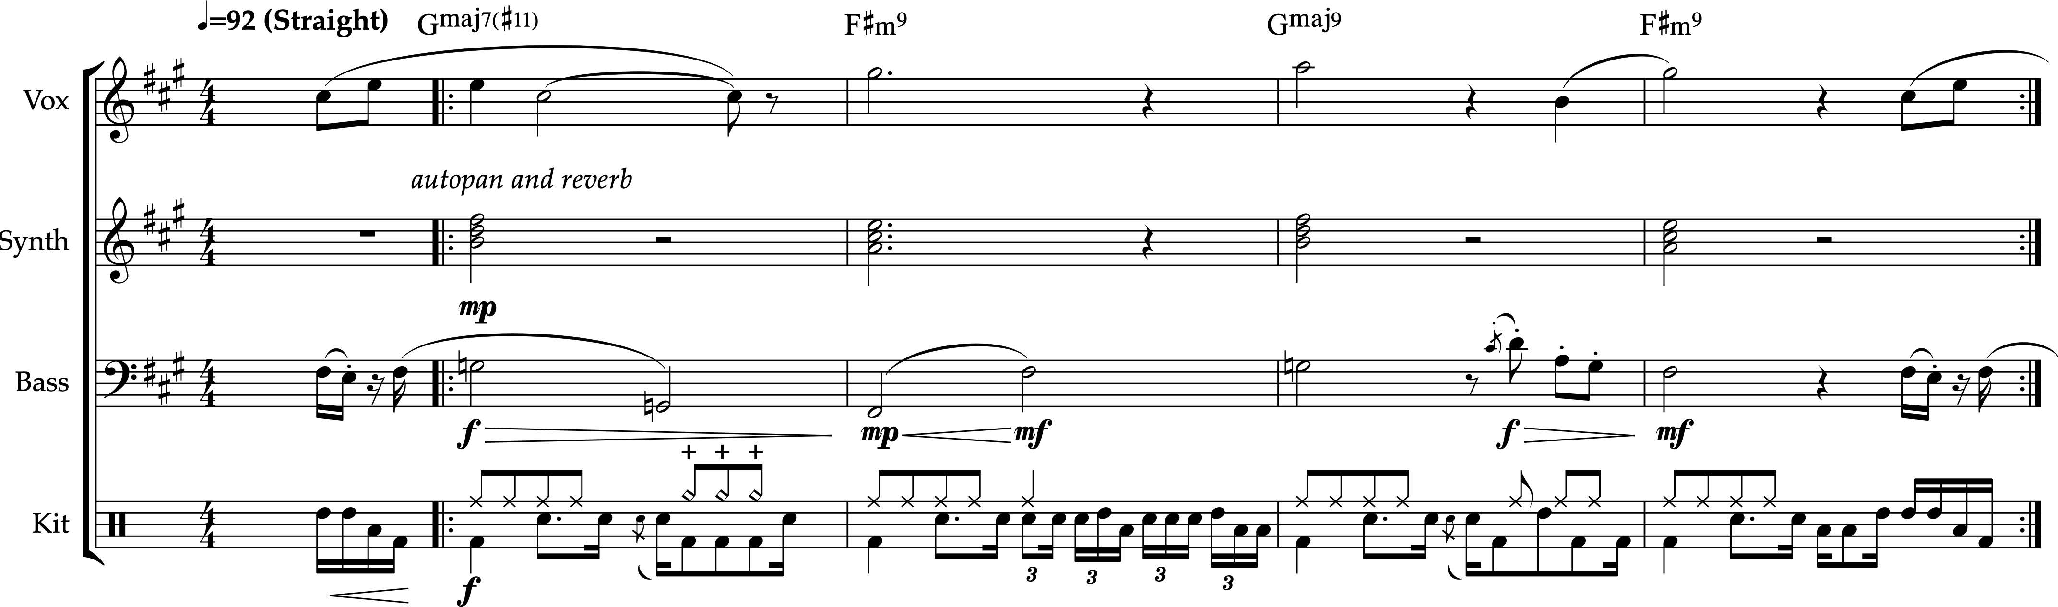
\includegraphics[width=\textwidth]{images/figures/chp 02/020031onebeermain.pdf}
        \caption{Snapshot of Madlib's second sample in ``One Beer,'' 0:20--0:31.}
        \label{fig:onebeermain}
    \end{figure}

The texture's most drastic change comes from the drum's rhythmic complexity in this sample.
Along with the harmony, the drums are thicker and more active, using distinctive fills and 
striking timbres throughout the four bar loop; this culminates in the prominence of the 
two-beat long triplet eighth fill in m. 2 of Figure~\ref{fig:onebeermain}. As Schloss notes,
producers often choose their samples based on the aesthetic delight they experience concerning
timbre, especially drum timbres.\footnote{
    \autocite[141--143]{josephgschlossMakingBeatsArt2004}.} 
Certainly, this second section luxuriates in the sonic quality of the drums.

Comparing the texture, harmony, and groove of each of Madlib's samples illustrates how internally
varied ``One Beer'' is. Although Madlib makes use of some of the methods of altering 
samples\textemdash particularly, choking the sample to delineate sectional transitions\textemdash
his primary method of introducing variety in the main part of ``One Beer'' is through the 
juxtaposition of the two lead samples. Juxtaposing musical elements in this manner aligns with 
Wilson's heterogeneous sound-ideal, particularly because of the  rhythmic clash and  timbral
stratification across sample boundaries.\footnote{
    \autocite[329--329]{ollywilsonHeterogeneousSoundIdeal1992}.}

The final skit section of ``One Beer'' functions as a culmination of Madlib's stylistic 
juxtapositions. The skit's music is built from a looped portion of the soundtrack to ``Dr. Doom,
Master of the World,''  an episode of the 1981 animated \textit{Spider-Man} television series. He
combines dialogue from this episode with another selection from ``The Fantastic Four Meet Dr. 
Doom,'' a 1978 episode of \textit{The New Fantastic Four}. Beneath this, Madlib improvises a 
through-composed drum sequence beholden to the boom-bap structure of kick and snare ubiquitous
in hip-hop. All in one track, Madlib draws on a ``rich assortment of multimedia borrowings, 
references, and parodies that operate in hip-hop music as a whole.''\footnote{
    \autocite[42]{joannademersSampling1970sHipHop2003}.} 
Juxtaposition is his method  of sounding DOOM's alternative identity.

\phantomsection
\subsection*{\centering Kendrick Lamar's ``Rigamortus''}
\addcontentsline{toc}{subsection}{Kendrick Lamar's ``Rigamortus''}

    \begin{table}[ht]
        \centering
            \begin{tabular}{|c|c|c|c|l|}
                \hline
                Section  & Timecode & Duration & Sample        & Note \\ \hline
                Intro    & 0:00     & 4 bars   & ``The Thorn'' & \\ \hline
                Hook     & 0:10     & 6 bars   & ``The Thorn'' & Full sample plays \\ \hline
                Verse 1A & 0:27     & 12 bars  & ``The Thorn'' & \\ \hline
                Verse 1B & 0:59     & 10 bars  & ``The Thorn'' & Improvisatory sample choking \\ \hline
                Hook     & 1:26     & 6 bars   & ``The Thorn'' & Lead sample slips backwards \\ \hline
                Verse 2A & 1:43     & 6 bars   & ``The Thorn'' & \\ \hline
                Verse 2B & 2:04     & 8 bars   & ``The Thorn'' & Alternating sample choking \\ \hline
                Hook     & 2:31     & 6 bars   & ``The Thorn'' & Improvisatory sample choking\\ \hline
            \end{tabular}
        \caption{Condensed roadmap to Kendrick Lamar and Willie B's ``Rigamortus.''}
        \label{tab:rigamortus}
    \end{table}

On ``Rigamortus,'' Willie B and Sounwave use Willie Jones  III's up-tempo jazz track ``The Thorn''
as the lead sample (0:13-0:20 of Jone's recording). Jones' combo groups simple quadruple meter 
into 3+3+2 beat divisions to underscore a saxophone and trombone theme that ends with a pickup
figure. This texture is detailed in Figure~\ref{fig:thethornfull}, which highlights boxes the
pickup in red.

    \begin{figure}[ht]
        \centering
        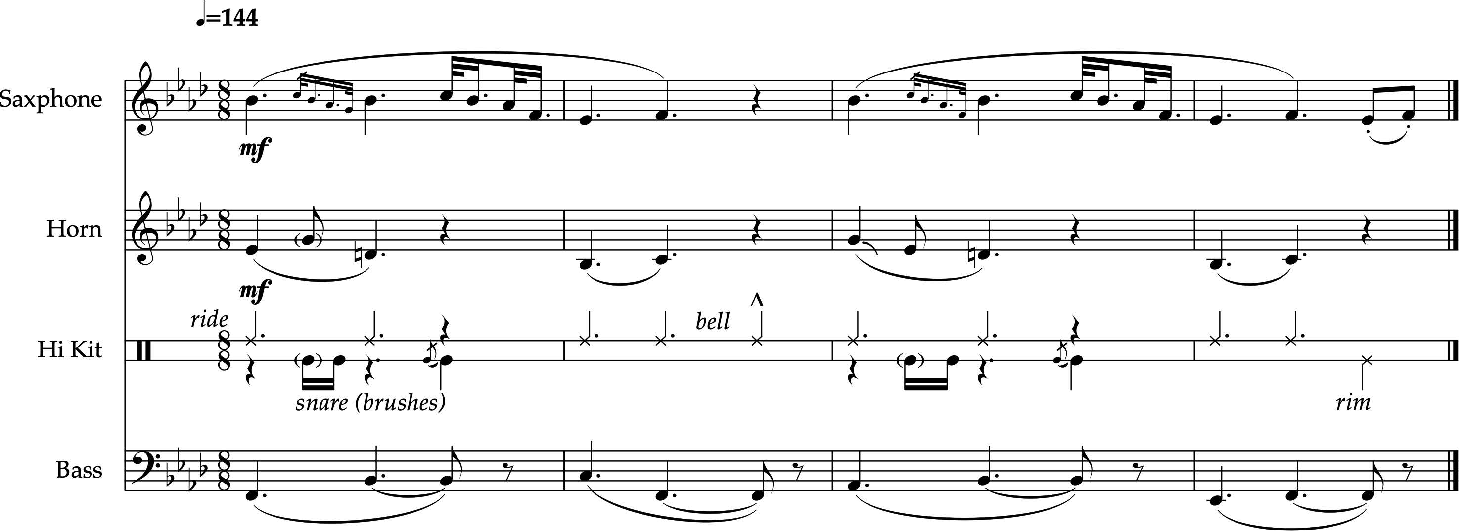
\includegraphics[width=\textwidth]{images/figures/chp 02/013020thethornfull.pdf}
        \caption{Snapshot of the sampled portion of ``The Thorn,'' 0:13--0:20.}
        \label{fig:thethornfull}
    \end{figure}

Kendrick's track begins with a minimally-altered version of the first two measures of the 
sample. The producers change it by filtering out the low end and pitching the sample up 
slightly  sharper than four semitones. In its new context, the two-bar phrase sounds as a
one-bar unit within a down tempo hip-hop context. Eight bars later, the full four-measure
sample is presented beneath Lamar's hook as a two-bar unit.\footnote{
    Table~\ref{tab:rigamortusfull} shows the moment where the full sample enters, notated
    as \textit{``The Thorn'' II}.}
Within the first verse, Willie B and Sounwave also layer in a drum sequence and sub bass 
drone on a low A using a filter sweep to demarcate their entrances. 
Figure~\ref{fig:rigamortusnoslip} shows the relationship of the sample (now in rhythmic
diminution) to the other elements of the musical texture; this structure repeats unchanged 
from 0:43-0:55, with only slight choking of the lead sample.

The musical additions recontextualize ``The Thorn'' a single A minor chord and simple quadruple
groove. Together, the sample, added drums, and bass each help ground the listener within Lamar's
complexities of vocal delivery and form, which frequently shift around throughout ``Rigamortus.''
Specifically, Lamar's vocals complicate form with shifts in text and delivery. In Verse 2, Lamar
briefly recapitulates the ``He Dead!'' call-and-response text from the hook, bisecting the verse.
He also restates the hook text at the beginning of Verse 2A, repeating ``Got me breathin' with 
dragons'' to set up a new rhyme structure and flow in the second verse. At the close of the Verse
2B, Lamar modulates into a higher and more rhythmically intense register, one that he identifies with 
his ``Gemini'' alter-ego.\footnote{
    \cite{chrismenchTrackingManyVoices2017}.}
The producers thus create contrast through simplicity by using discrete, simplistic musical elements.

\begin{figure}[ht]
    \centering
    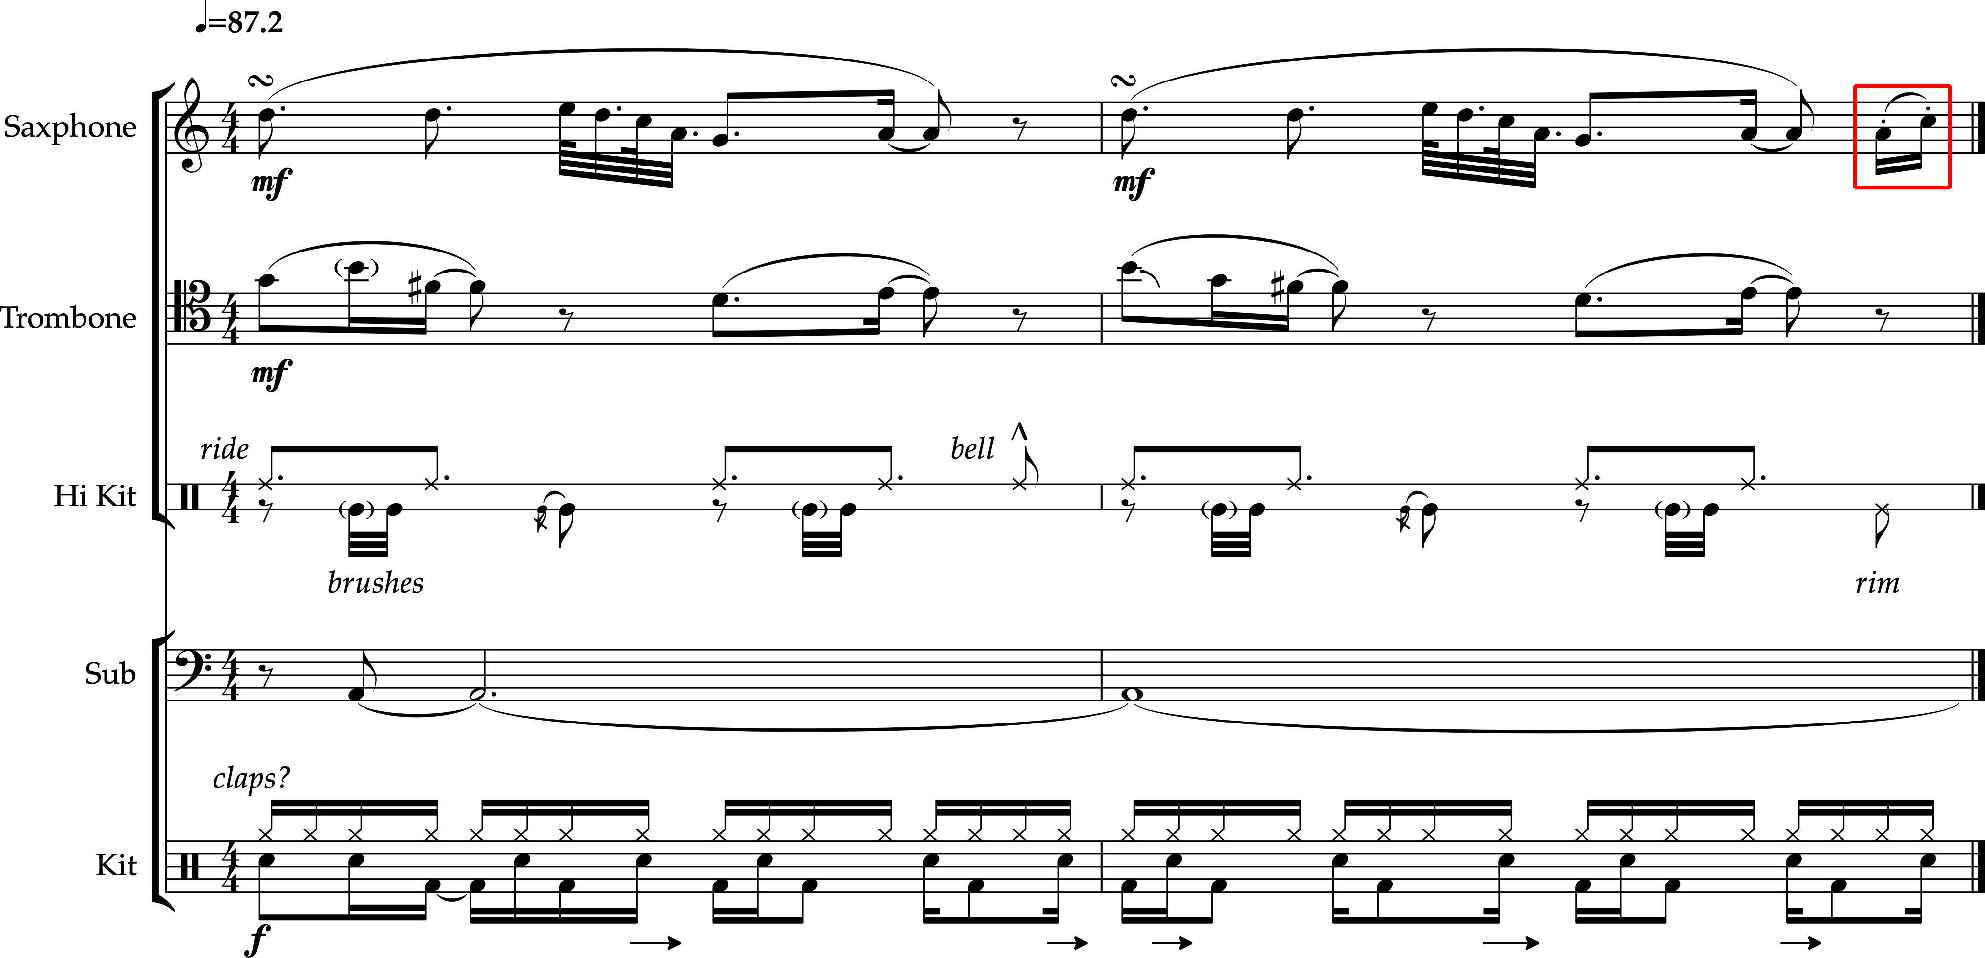
\includegraphics[width=\textwidth]{images/figures/chp 02/043053rigamortusnoslip.pdf}
    \caption{Snapshot of the first verse in ``Rigamortus,'' 0:43--0:55.}
    \label{fig:rigamortusnoslip}
\end{figure}

Despite using samples and loops in a simplistic way, Willie B and Sounwave vary their them
subtly within the repeating texture. As Table~\ref{tab:rigamortus} notes, sample choking
features heavily in this track; the lead sample from ``The Thorn'' rarely sounds intact once
introduced. With Lamar's vocals taking on the ``tendency to fill up sonic space'' of Wilson's
heterogeneous sound-ideal,\footnote{
    \autocite[328]{ollywilsonHeterogeneousSoundIdeal1992}.} 
the producers choke the sample because it removes elements from the texture, and they employ
the technique most drastically when Lamar's vocals reach an apex in Verse 2B. From 2:06-2:18,
the lead sample drops out for measures at a time time, leavin space for Lamar's flow. Thus,
their implementation of sample choking exists in conversation with Lamar's musical decisions.

\begin{figure}[htp]
    \centering
    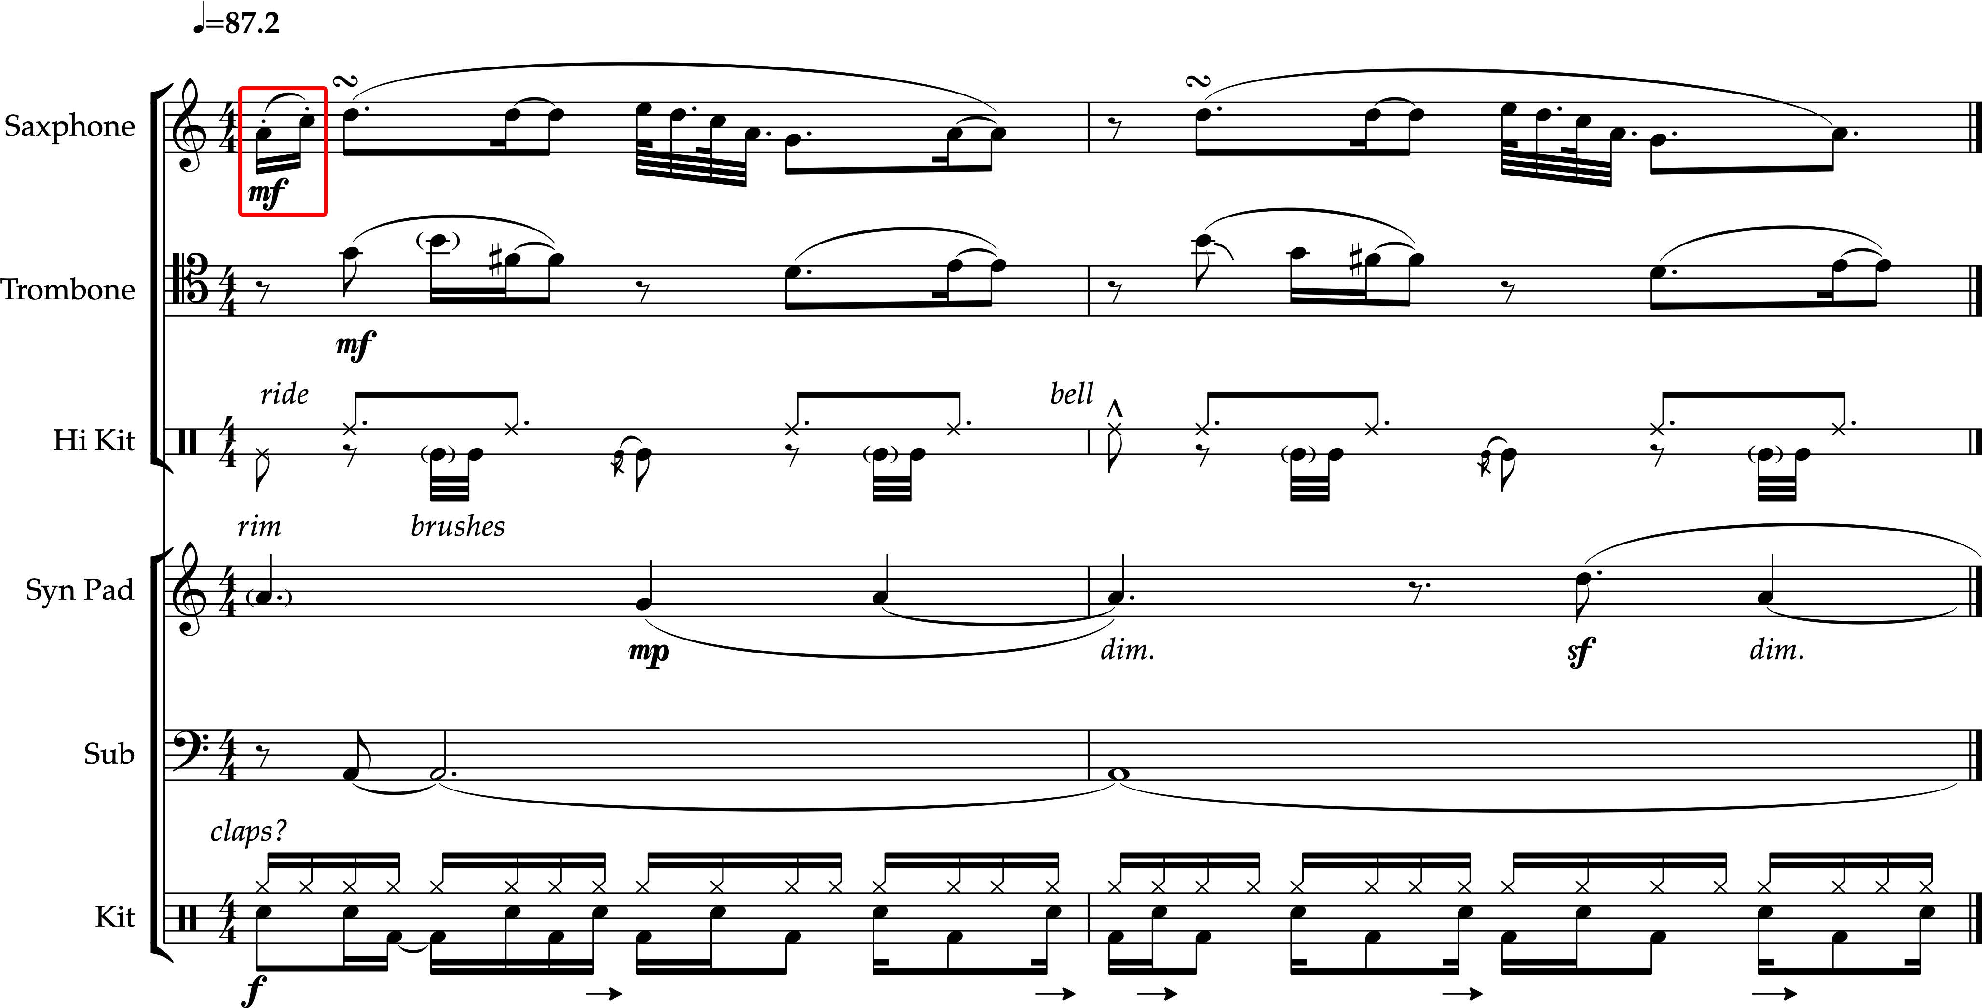
\includegraphics[width=\textwidth]{images/figures/chp 02/126137rigamortusslip.pdf}
    \caption{Snapshot of the first hook in ``Rigamortus,'' 1:26--1:37.}
    \label{fig:rigamortusslip}
\end{figure}

More subtly, the producers slip the lead sample to alter the beat in ``Rigamortus.'' Through
expressive, delayed re-triggering, the microrhythmic relationship between musical elements from
``The Thorn'' and the producers' additions exist throughout the work in a state of rhythmic 
flux.\footnote{
    My theory of sample slippage dovetails with Anne Danielsen's work on the Beat Bin and 
    rhythmic tolerance (see \autocite[29\textit{ff}.]{annedanielsenHereThereEverywhere2016}. 
    The affective result of these shifts creates a listening experience akin to phasing, 
    as samples (albeit sonically discrete ones) move in and out of sync with each other.}
Where the pickup gesture in the saxophone (boxed in red in Figures~\ref{fig:thethornfull}
and~\ref{fig:rigamortusnoslip}) fell at the metrical end of the loop when it was first heard,
the pickup gesture falls in different metrical positions throughout the hook, displaced from
its original position in the groove. As Figure~\ref{fig:rigamortusslip} shows, the pickup 
figure sounds on the downbeat. The drum sequence and Lamar's call-and-response vocal enter 
on the downbeat\textemdash and the saxophone, trombone and sub-bass enter with them. The 
producers' use of slippage, then, allows for a sample, which is typically sonically fixed,
to become rhythmically fluid.

Willie B and Sounwave's production on ``Rigamortus'' challenges a listener's sense that 
the lead sample on the track is uniformly repetitive. While choking and slipping serve as
their primary methods of altering the sample itself, they also create variety in the beat
through the use of digitally-recorded loops, layering in and out of the mix throughout the
track. These loops are all used in conversation with Lamar's vocal delivery, helping to 
create an even greater sense of variety within the musical texture. Compared to Madlib's 
approach to beatmaking, which created variety primarily through the juxtaposition of 
disparate samples, Willie B and Sounwave track new elements around the lead sample, 
widening the sample's context. This links the practice of creating variety in sample-based
hip-hop to another style of production: live-tracked recording.

%\clearpage
\section{Live-Tracked Case Studies}
The second half of this chapter shifts in focus from beats that are sample-based to beats that are
live-tracked. While the distinction between these approaches remains helpful to identifying and describing
the components of a musical texture, it is not a distinction that holds significance beyond this. 
Schloss's ethnographic work in the early-to-mid 2000s Seattle hip-hop scene leads him to the conclusion
that ``the distinction between sample-based and non-sample-based hip-hop is a distinction in
genre.''\footnote{\cite{josephgschlossMakingBeatsArt2004}, 5.} I do not intend to bring in 
such a distinction.

While Schloss's framework may help to explain works in early 2000s underground hip-hop, it becomes
increasingly problematic within modern approaches to music making. When a beat is created in a DAW, 
the distinction between sampling vinyl, using pre-recorded audio or MIDI loops, and live-tracking an
instrument becomes less drastic than within older recording hardware. With the following examples, I aim
to demonstrate that beats are not underground because of the means of generating musical material, but 
rather because of the manipulation of material thereafter.

\phantomsection
\subsection*{\centering Milo's ``Rabblerouse''}
\addcontentsline{toc}{subsection}{Milo's ``Rabblerouse''}

\begin{table}[ht]
    \centering
        \begin{tabular}{|c|c|c|c|l|}
             \hline
            Section & Timecode & Duration & Sample                   & Note \\ \hline
            Intro   & 0:00     & 4 Bars   &                          & Rhodes extends over boundary \\ \hline
            Verse   & 0:08     & 24 Bars  &                          & \\ \hline
                    & 0:14     &          &                          & Drum glitch \\ \hline
                    & 0:36     &          &                          & Drum glitch, bass recomp. \\ \hline
            Outro   & 0:56     & 4 Bars   &                          & Glich, recomp., and choking \\ \hline
                    & 1:03     &          & \textit{Soulcallibur II} & \\ \hline
        \end{tabular}
    \caption{Condensed roadmap to Milo and Kenny Segal's ``Rabblerouse''}
    \label{tab:rabblerouse}
\end{table}

Kenny Segal's instrumental for ``Rabblerouse'' creates variety as a complement to Milo's emceeing.
As shown in Table~\ref{tab:rabblerouse}, ``Rabblerouse'' consists of a single twenty-four-bar verse
framed by an intro and outro. The track does not end with music but sounds a vocal sample of the 
video game character Yoshimitsu from \emph{Soulcallibur II}, saying ``overconfidence is the greatest
enemy'' before giving a battle cry. The sample links  ``Rabblerouse'' as an introductory song fragment
to Milo's full LP, \emph{So The Flies Don't Come}. It both propels the listener into the downbeat of 
the second track, ``Souvenir,'' and links thematically to a line Milo delivers in the penultimate track,
``Napping Under the Echo Tree,'' where Milo gives himself the epithet ``Yoshimitsu of Boyle Heights.''
With both sample selection and music, Segal uses ``Rabblerouse'' to create instability, urging the 
listener on toward the album as a whole.

Several elements contribute to the fragmentary nature of this opening track. Its primary melodic
component is and unconventional six-bar chord loop, played in staccato quarter notes on a Fender 
Rhodes. Although functional in E Dorian, the expansional loop sounds unresolved.\footnote{
    \cite{kyleadamsHarmonicSyntacticMotivic2020}. Adams does not make it a requisite condition
    of the expansional harmonic category to function as a complete phrase, although he notes that
    it commonly will.} 
The C\#$^{sus4}$ that ends the loop, rather than resolving the suspension down, cycles back to a
similarly-voiced E$^{sus4}$. The stability of this chord loop is also challenged by Milo's vocal 
entrance, which comes after a more-conventional four bars. The Rhodes progression extends over
this formal boundary, offsetting the downbeats being projected by rapper and producer.

    \begin{figure}[ht]
        \centering
        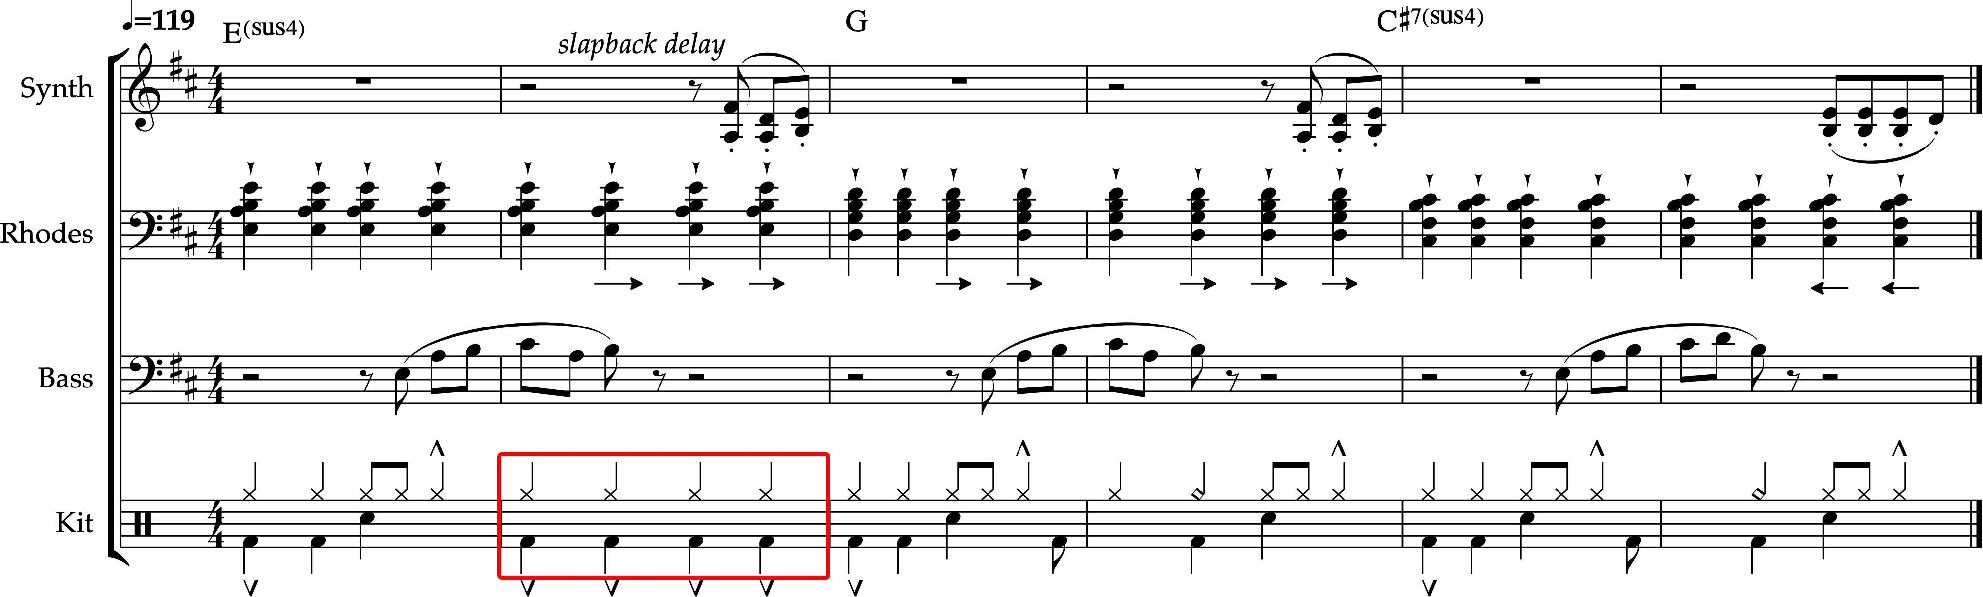
\includegraphics[width=\textwidth]{images/figures/chp 02/012023rabblefirstglitch.pdf}
        \caption{Snapshot of the first drum glitch in ``Rabblerouse,'' 0:12--0:23.}
        \label{fig:rabblefirstglitch}
    \end{figure}

Segal uses glitch as a method of alteration in response to this dissonance between the agogic
stress of the rapped text and the beat. Boxed in red in Figure~\ref{fig:rabblefirstglitch}, 
he alters where the loop begins, reworking the loop's metrical accent. In m.~2, four quarter-note
kick and hi-hat hits repeat for a full bar; here, Segal has likely selected a portion of the drum
loop in his DAW and duplicated it four times, restarting the loop in m. 3. This instance underscores
the textual beginning of a new idea: Milo begins ``The wordsmith gets knee-deeper, beleaguered'' and
Segal's glitch transforms the start of the phrase into an upbeat, so that ``deeper'' becomes the 
strongest metric point of the phrase. This glitch reworks the alignment of the drum loop and rapper,
a partial corrective to the dissonance between Milo's entrance and the loop.

    \begin{figure}[ht]
        \centering
        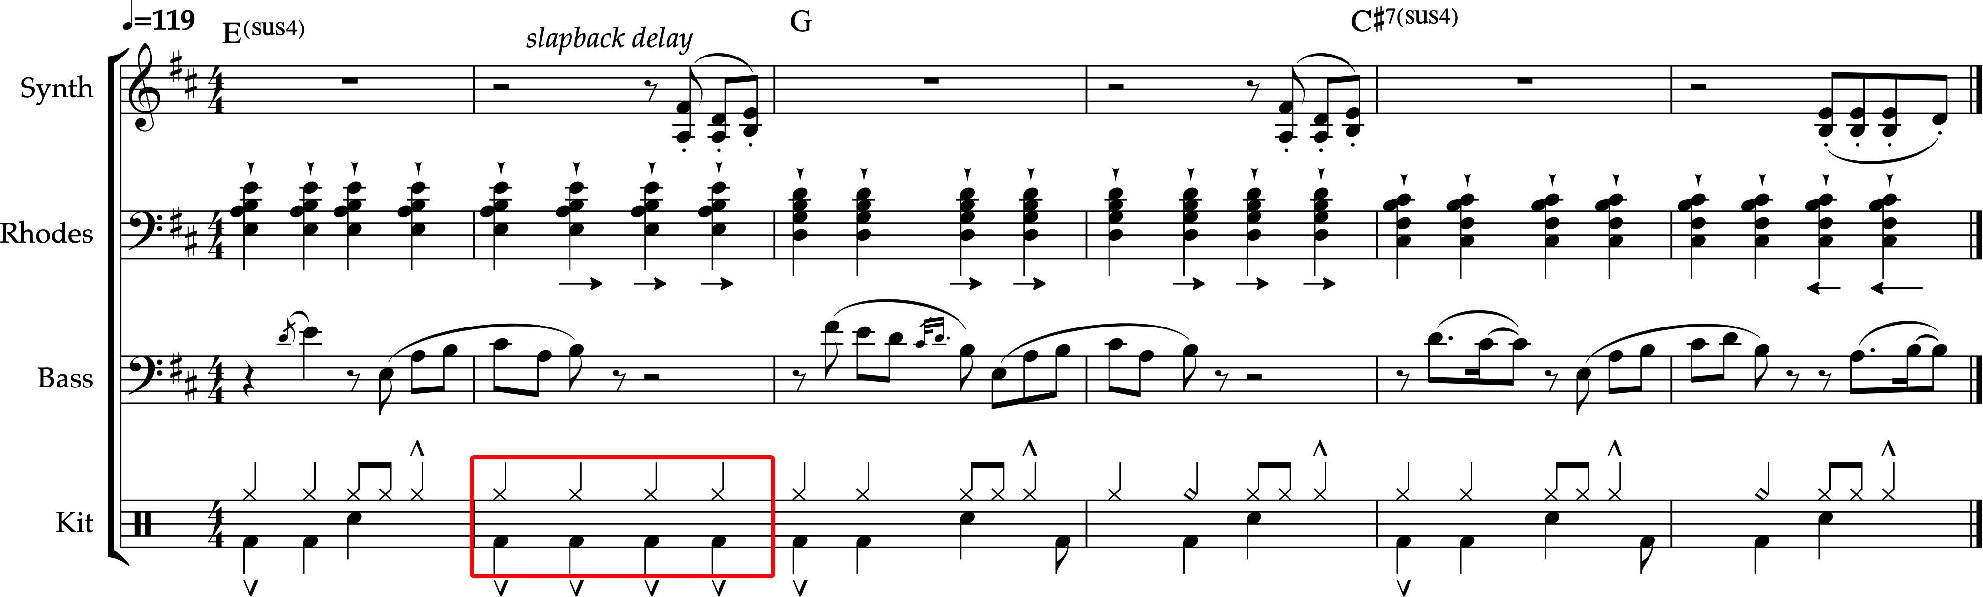
\includegraphics[width=\textwidth]{images/figures/chp 02/036048rabblesecondglitch.pdf}
        \caption{Snapshot of the second drum glitch in ``Rabblerouse,'' 0:36--0:48.}
        \label{fig:rabblesecondglitch}
    \end{figure}

A parallel instance to the first glitch occurs from 0:36-0:48, and its onset is further complicated
by Segal's use of a bass recomposition. Figure~\ref{fig:rabblesecondglitch} shows the loops in this 
moment, with the changes to the bassline implemented by bassist and frequent collaborator of Segal's, 
Mike Parvizi. Parvizi decorates the originally sparse bass lines that begin mid-measure with sleek,
syncopated melodic lead-ins. This busies the texture while Segal uses another glitch accentuate
mm. 2-3. Milo's text (``suits of armor for suicide note authors'') again becomes a point of agogic 
stress, but around this measure, Parvizi's basslines increase the number of rhythmic onsets within 
the measure, thereby increasing heterogeneity.\footnote{
    \cite{ollywilsonHeterogeneousSoundIdeal1992}, 328. Wilson describes the ``tendency to create 
    rhythmic musical events clash or disagreements of accents'' as a component of the ideal.}

Glitch becomes a method of constructing cohesivity at the track's close. As Milo comes to the end
of his verse, Segal uses the same downbeat-repeating drum glitch, pairing it with a glitch that 
extends the E$^{sus4}$ harmony. This point of stasis, though harmonically unresolved, allows
for the listener to hear rhythmic unification for a brief instant, before the texture dissolves and
the Yoshimitsu sample is triggered. Drawing on several methods of altering loops in the beat, Segal
brings together the many fragmentary, disparate pieces of the loop for a brief moment to set a 
listener up for what's to come on the record overall.

Segal's fragmentary aesthetic on ``Rabblerouse'' sounds as a mode of alterity because it is uncommon
for a hip-hop beat not to function as a closed loop. The metric dissonance projected from the 
beginning does not resolve by the track's end, necessarily drawing a listener in to the text function
and pointing  towards the remaining tracks on the album. This beat is unstable alone, but functions 
cohesively with the sonic palette of Milo's LP \textit{So The Flies Don't Come} as a whole. This 
technique is predicated  upon an interest in lyricism and album cohesivity propagated within the
underground hip-hop scene.

\phantomsection
\subsection*{\centering billy woods' ``Checkpoints''}
\addcontentsline{toc}{subsection}{billy woods' ``Checkpoints''}

\begin{table}[ht]
    \centering
    \begin{tabular}{|c|c|c|l|}
        \hline
         Section      & Timecode & Duration & Note                          \\ \hline
         Intro        & 0:00     & 8 Bars   & Guitar anacrusis choked       \\ \hline
         Verse 1A     & 0:26     & 22 Bars  & Vocal, synth  anacrusis       \\ \hline
                      & 0:40     &          & Guitar, synth recomp          \\ \hline
         Verse 1B     & 1:06     &          & Synth, drum recomp            \\ \hline
         Interlude 1  & 1:40     & 4 Bars   &                               \\ \hline
         Hook?        & 1:51     & 4 Bars   & All parts anacrusis           \\ \hline
         Interlude 2  & 2:06     & 4 Bars   &                               \\ \hline
         Verse 2      & 2:20     & 15 Bars  & Synth anacrusis glitch        \\ \hline
         
    \end{tabular}
    \caption{Condensed roadmap to billy woods and Kenny Segal's ``Checkpoints.''}
    \label{tab:checkpoints}
\end{table}

Segal served as the beatmaker for billy woods' ``Checkpoints,'' as well as the \textit{Hiding Places}
LP which houses it. Comparing his production across projects for two different emcees shows how Segal
responds to both the artist and the work itself, articulating identity uniquely for each. Compared to
``Rabblerouse,'' Segal's instrumentation on ``Checkpoints'' is at once sparser and more timbrally intense;
the choice to use distored, low-register electric guitar played on neck pickups matches woods' more highly
energetic emceeing. Likewise, Segal responds to formal sections of text, working with woods to create
formal contrast. Table~\ref{tab:checkpoints} shows the main formal features: a brief introduction,
followed by two verses of varying lengths, which are divided by an interlude and short hook-like
vocal section.

A significant features of the beat's construction is the use of anticipation and anacrusis.\footnote{
    I use the term anacrusis as opposed to pickup here because the track does not contain
    the final two beats. In the fifteenth bar of the second verse, woods raps through beat two,
    before  a static signal sounds for a beat, cutting off before beat four.} 
Underscoring woods' entrances which typically enter two bars before a downbeat, Segal introduces all
musical elements in the two beats preceding the expected loop onset. Figure~\ref{fig:checkpointsintro} 
shows each element's entrance from 0:26-0:39 when woods' first verse enters. Segal employs a high synth
leadline paired with the guitar loop outlining an F-sharp power chord. An eighth note before the downbeat,
the guitar oscillates to a G harmony, supported by an anticipation in the kick drum. These anticipations
create some rhythmic disorientation in contrast to the snare drum, which hits in its expected position
on the backbeats.

    \begin{figure}[ht]
        \centering
        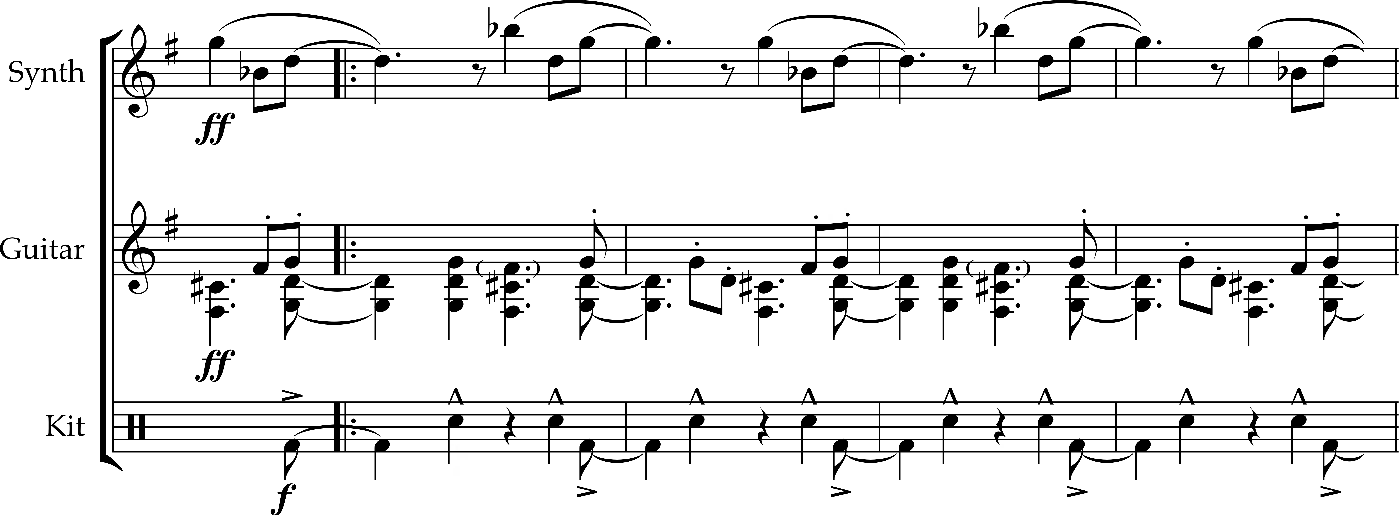
\includegraphics[width=\textwidth]{images/figures/chp 02/026039checkpointsintro.pdf}
        \caption{Snapshot of the beginning of the first verse of ``Checkpoints,'' 0:26--0:39.}
        \label{fig:checkpointsintro}
    \end{figure}

Segal introduces variety into the texture using two recompositions. His drum recompostion, shown 
in Figure~\ref{fig:checkpointsmain}, divides the first verse  into two eleven-bar units. Following
the structure outlined by the kick-snare pattern up to this point, a crash cymbal enters with the 
downbeat anticipation in the kick, and the same sample sounds a step  higher along with an open 
hi-hat sample above the snare's backbeats. This rock-like groove serves as Segal's means of creating
variation at an unexpected point of formal division.

    \begin{figure}[ht]
        \centering
        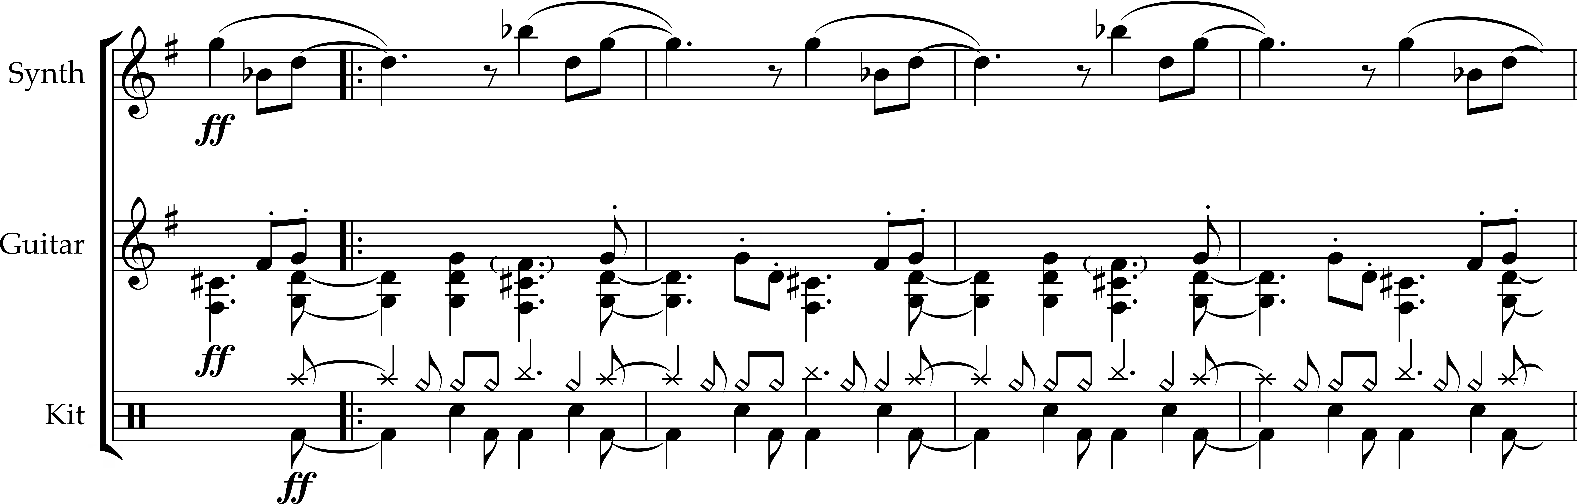
\includegraphics[width=\textwidth]{images/figures/chp 02/106119checkpointsmain.pdf}
        \caption{Snapshot of the drum recomposition in ``Checkpoints,'' 1:06--1:19.}
        \label{fig:checkpointsmain}
    \end{figure}

Even with woods' vocal delivery signalling a change, the drum recomposition can catch the listener
off-guard. New additions to the drum sequence highlight irregularities in his placement of the 
kick-snare alteration and are added at a surprising moment in the form. On another level, Segal's
choice of drum timbre surprises a listener by challenging their sense of genre. Throughout 
\textit{Hiding Places}, Segal sought out ``distorted guitars and psych-rock timbres,'' playing with
stylistic allusion on  tracks like ``Checkpoints,'' ``Spongebob,'' and ``Speak Gently.''\footnote{
    Quoted in \cite{backwoodzhiphopKennySegalPresents2019}.} 
On ``Checkpoints'' specifically, the full drum pattern alludes to rock while introducing variety.

    \begin{figure}[ht]
        \centering
        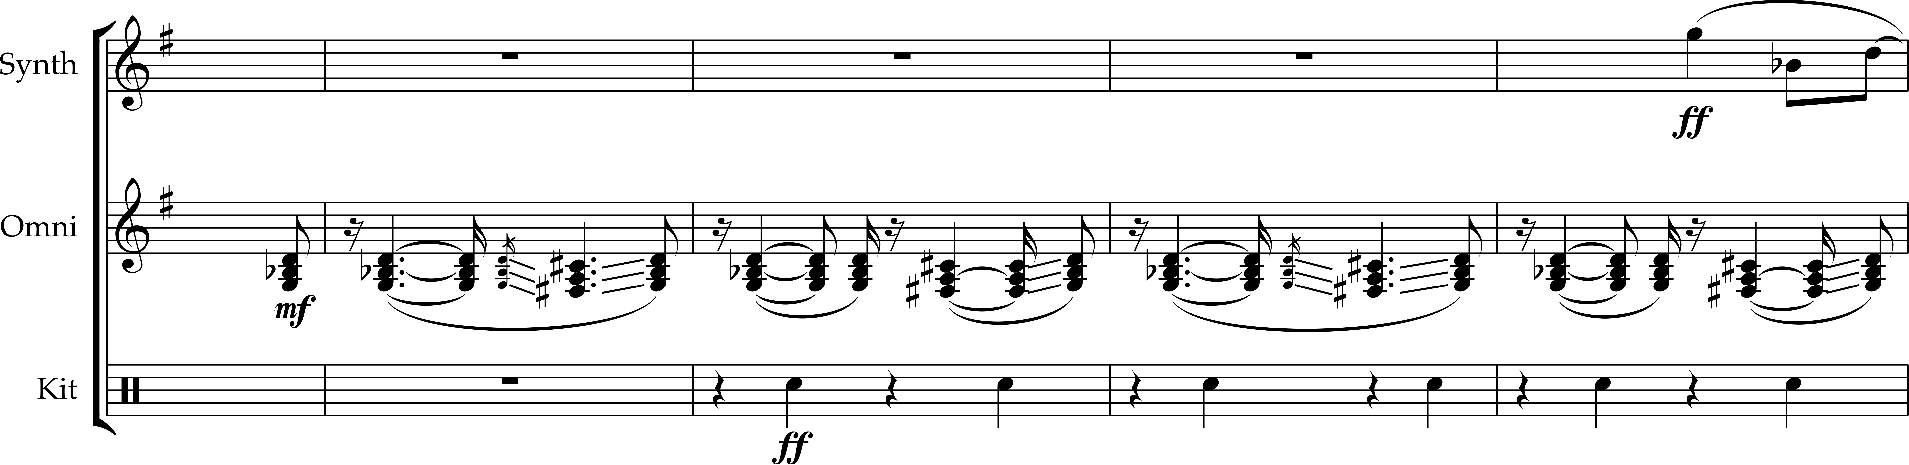
\includegraphics[width=\textwidth]{images/figures/chp 02/040053checkpointsrecomp.pdf}
        \caption{Snapshot of the chordal recomposition in ``Checkpoints,'' 0:40--0:53.}
        \label{fig:checkpointsrecomp}
    \end{figure}

Additionally, Segal recomposes the chord loop to introduce formal and textural variety. Figure
\ref{fig:checkpointsrecomp} shows its first entrance, midway through Verse 1A. Still in rhythmic 
anticipation of the downbeat, the chord loop switches from a guitar outlining G and F-sharp power
chords to a Suzuki Omnichord planing between G-minor and F-sharp minor triads in the same low-mid
layer. The paired range and voicing, as well as the similar rhythm used in the Omnichord's version,
challenges the sense that a new layer has entered, sounding more like a the timbre of the original
loop has changed.\footnote{
    This use of timbral shifts within a shared musical range creates an unblended, heterogeneous 
    quality within the chordal accompaniment, in keeping with Wilson's heterogeneous 
    sound ideal (see \autocite[329]{ollywilsonHeterogeneousSoundIdeal1992}.)}

Each time the chordal recomposition enters, Segal removes all other accompaniment before reintroducing
the snare and synth lead. This thinned out texture takes on two distinct formal roles: within the first
verse, Segal uses this recomposition to reduce the energy of the beat, making the drum recomposition
even more drastic when it re-enters with the guitar twenty seconds later. Between the two verses,
the recomposition signals a higher-order formal boundary. The four bars of text woods delivers that
Table~\ref{tab:checkpoints} denotes a \textit{Hook?} are offset by Omnichord interludes but underscored
by the more-fully orchestrated texture characteristic of the verses. This affords a certain weight to
the text of the four intervening bars; likewise, woods' text in that section has a certain thematic
weight to it.

Throughout ``Checkpoints,'' Segal uses  recompositions to create an internal variety within the song
form while playing with the broader, generic context of underground hip-hop. In his memory of 
mainstream rap history, the use of rock-like timbres in hip-hop has,  on occasion, yielded ``disastrously
wack results.''\footnote{
    \cite{backwoodzhiphopKennySegalPresents2019}.}
His choice to navigate this potentially-treacherous sonic territory reveals his willingness to re-purpose
sounds which have associations with normative, mainstream expectations. At the same time, the timbral
particularities of ``Checkpoints'' illustrate his desire to do so with specific aesthetic
and compositional ends in mind: namely, those linked to the textual, thematic, and vocal specificities
of woods' emceeing. Segal's primary concern as a  producer, then, seems to be sounding an identity
\emph{with} the emcee.

%\clearpage
\section{The Co-Creation of Underground Identity}
As a stylistic practice in underground hip-hop, producers work as coauthors in the creation of underground
identity with the emcee. Because their work is largely non-textual, underground producers use normative 
expectations for form and content in a hip-hop track as a basis for a type of sonic play that manifests
as heterogeneity within a hip-hop beat's construction. Underground producers create forms that are 
non-normative, articulating them through sample and loop juxtapositions, and ascribing formal rhetoric 
to different portions of the beat through their choice of sequencing. Within samples and loops, producers
create heterogeneity with a variety of techniques for manipulating  sound, four of which I have explored
in depth during this chapter. For the underground producer, formal and compositional variety functions
as a sonic metaphor for the non-normativity of the emcees who rap over these tracks.